\documentclass[11pt,a4paper]{article}
\usepackage[spanish]{babel}			%Encabezados automaticos en español
\usepackage{listings}				%Utilizar codigo de un programa
\usepackage{url}					%Ingresar url
\usepackage{graphicx}				%Ingresar imagenes
\usepackage[usenames,dvipsnames]{color}					%Libreria para colores
\usepackage{amsmath,amsfonts,amsthm} % Math packages for equations
\usepackage[hang, small, labelfont=bf, up, textfont=it]{caption} % Custom captions under/above tables and figures
\usepackage{float}
\setlength{\parskip}{12pt}			%espacio entre parrafo
\setlength{\parindent}{0pt}			%espacio de sangria
\usepackage{enumerate}
\usepackage{subfigure}

\usepackage{pdfpages}
\usepackage[left=4cm,right=3cm,top=4cm,bottom=3cm]{geometry}

\author{Brenda Yaneth Sotelo Benítez \\ 1565705}
\title{Optimización de flujo en redes\\ 
Portafolio}

\begin{document}
\maketitle 

\setlength{\parindent}{0cm}

\section*{Introducción}

En este reporte se recopilan las distintas tareas realizadas a lo largo de la unidad de aprendizaje de optimización de flujo en redes realizadas durante el período Enero-Junio 2019. Cada una de estas tareas contiene anotaciones con puntos a corregir, las cuales fueron tomadas en cuenta en la elaboración del portafolio. Se muestra cada tarea calificada y la respectiva tarea corregida si es necesario.  


\newpage

%---------------------------------------------------------
\section*{Tarea 1}
Al realizar esta práctica y recibir retroalimentación, los principales errores encontrados fueron de ortografía, falta de espacios al citar, de ambiente matemático y errores en la bibliografía. 

\newpage
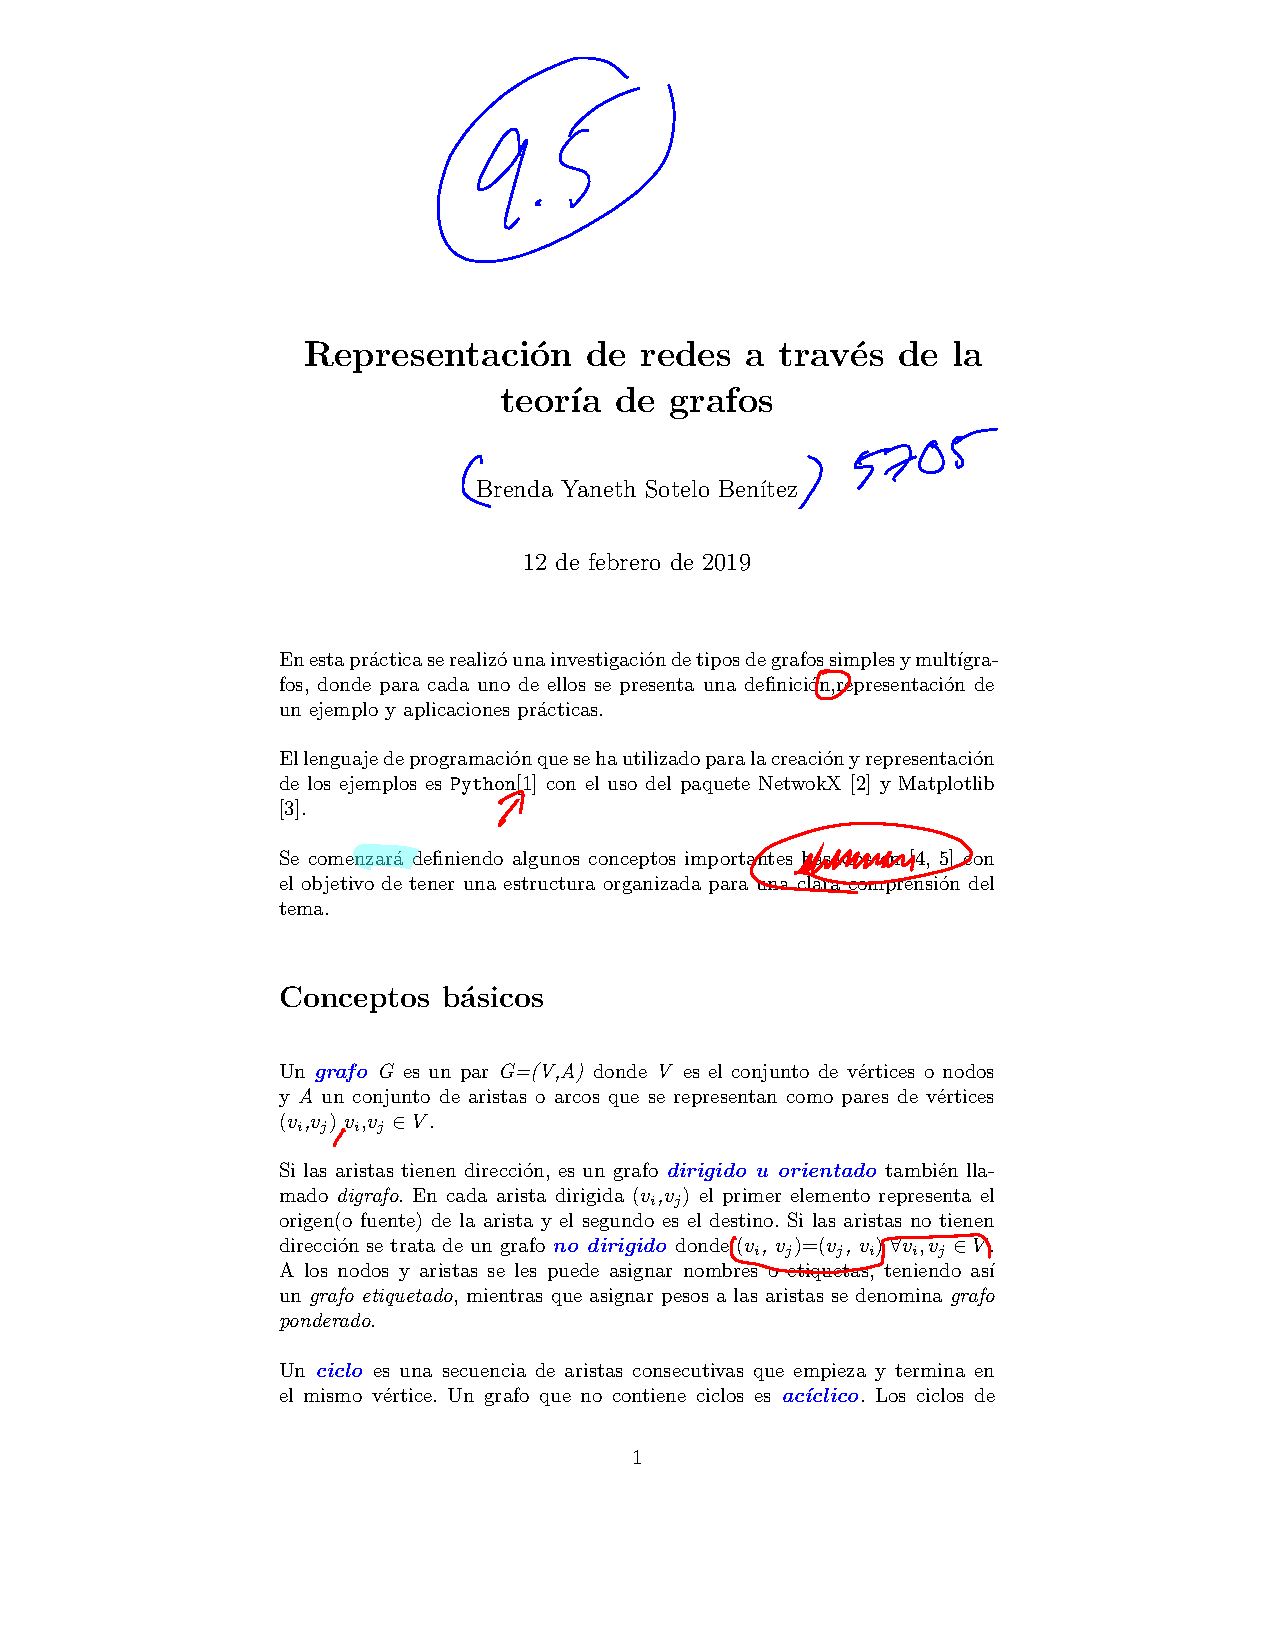
\includepdf[pages=-]{5705-1.pdf}
\newpage
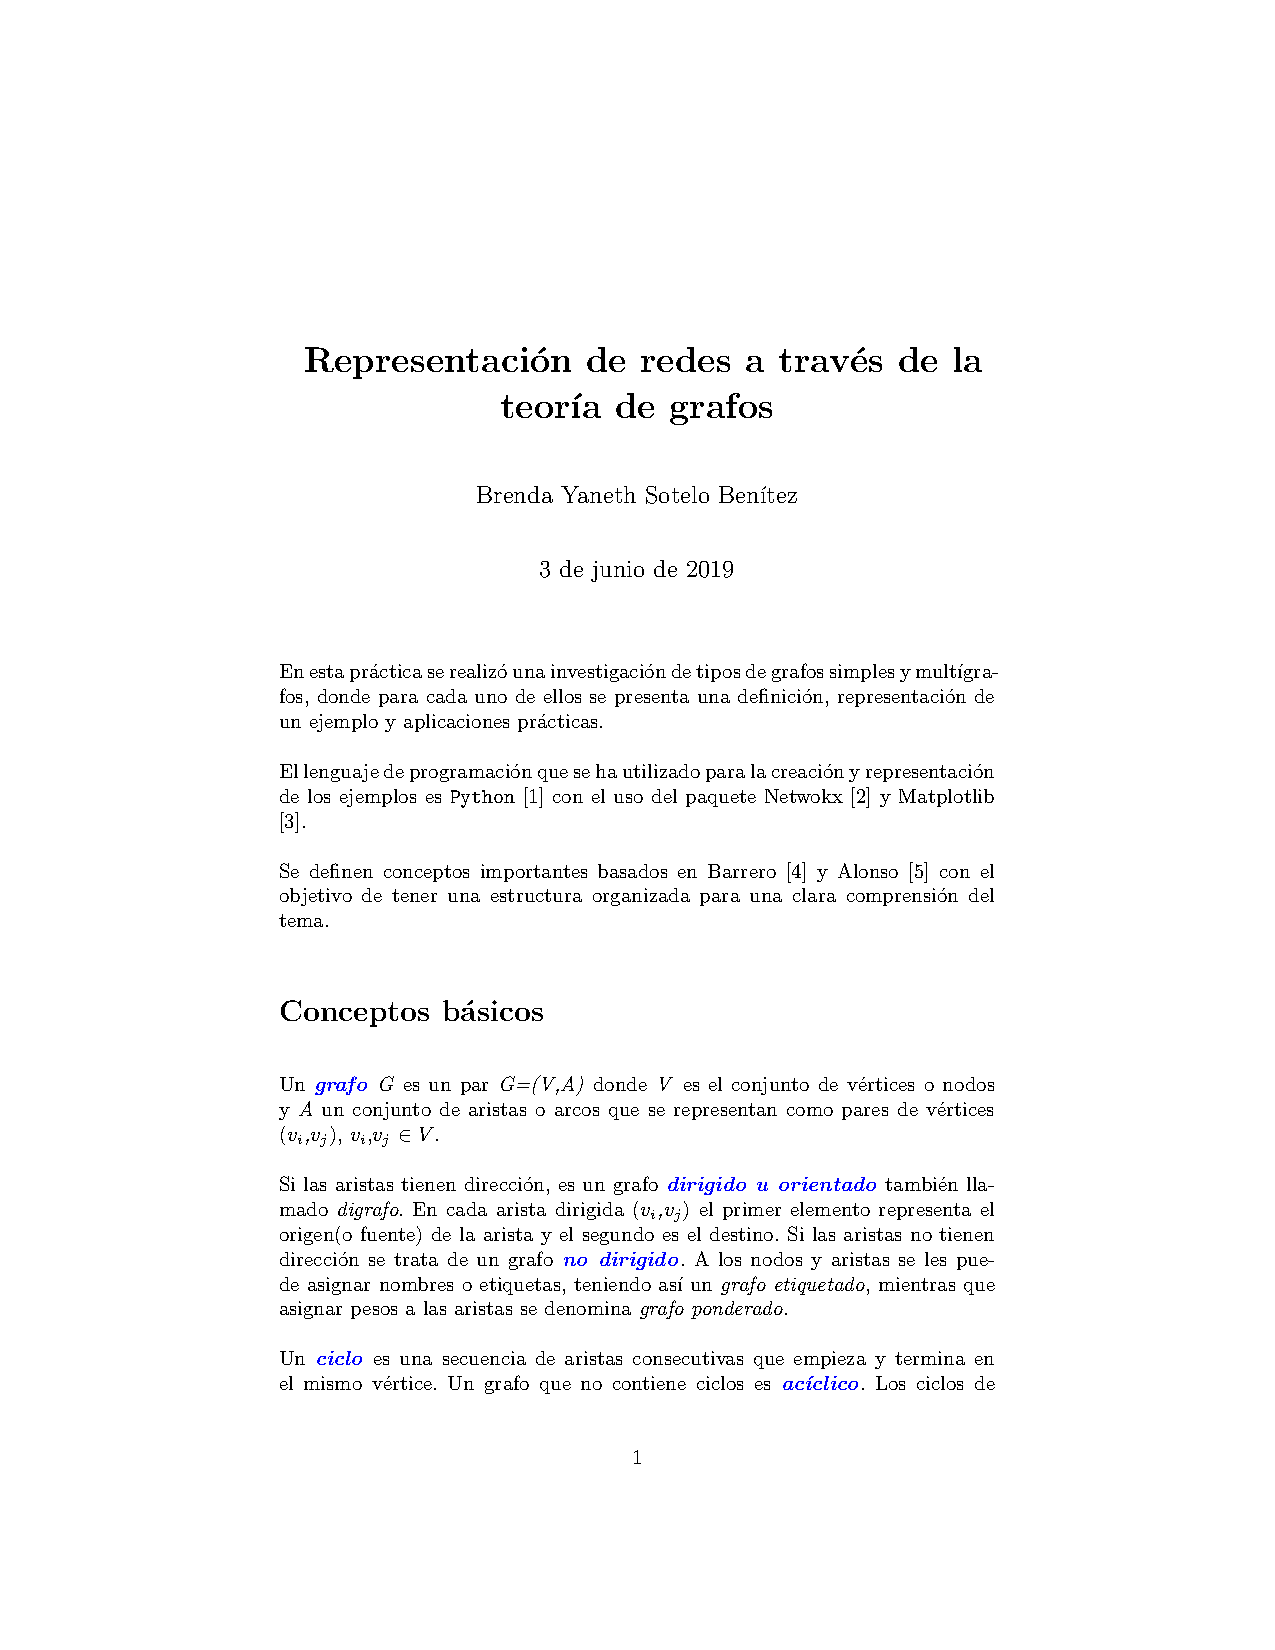
\includepdf[pages=-]{Tarea1_FR.pdf}
%---------------------------------------------------------

%---------------------------------------------------------
\section*{Tarea 2}

En esta práctica se realizaron pequeñas correcciones ortográficas y la correcta forma de citar.  Aún así se muestra la versión corregida de la tarea. 

\newpage
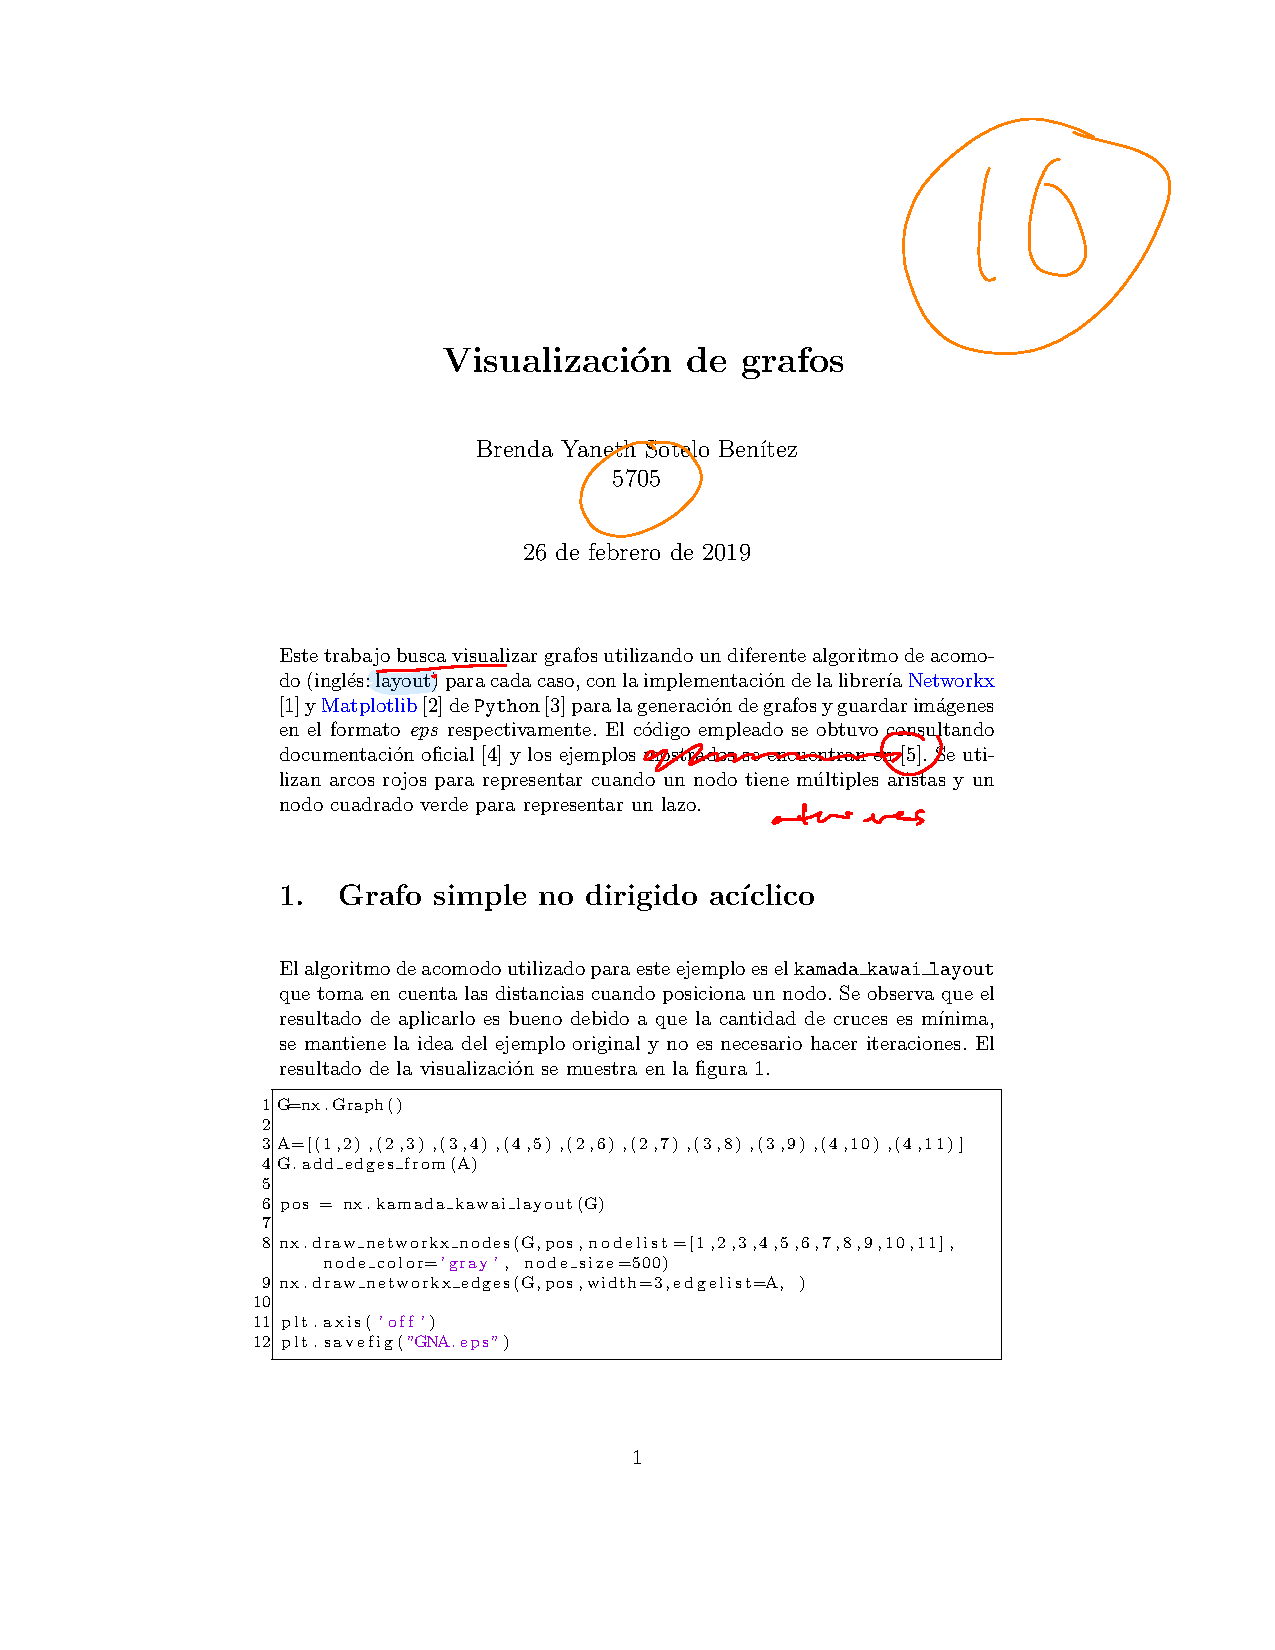
\includepdf[pages=-]{5705-2.pdf}
\newpage
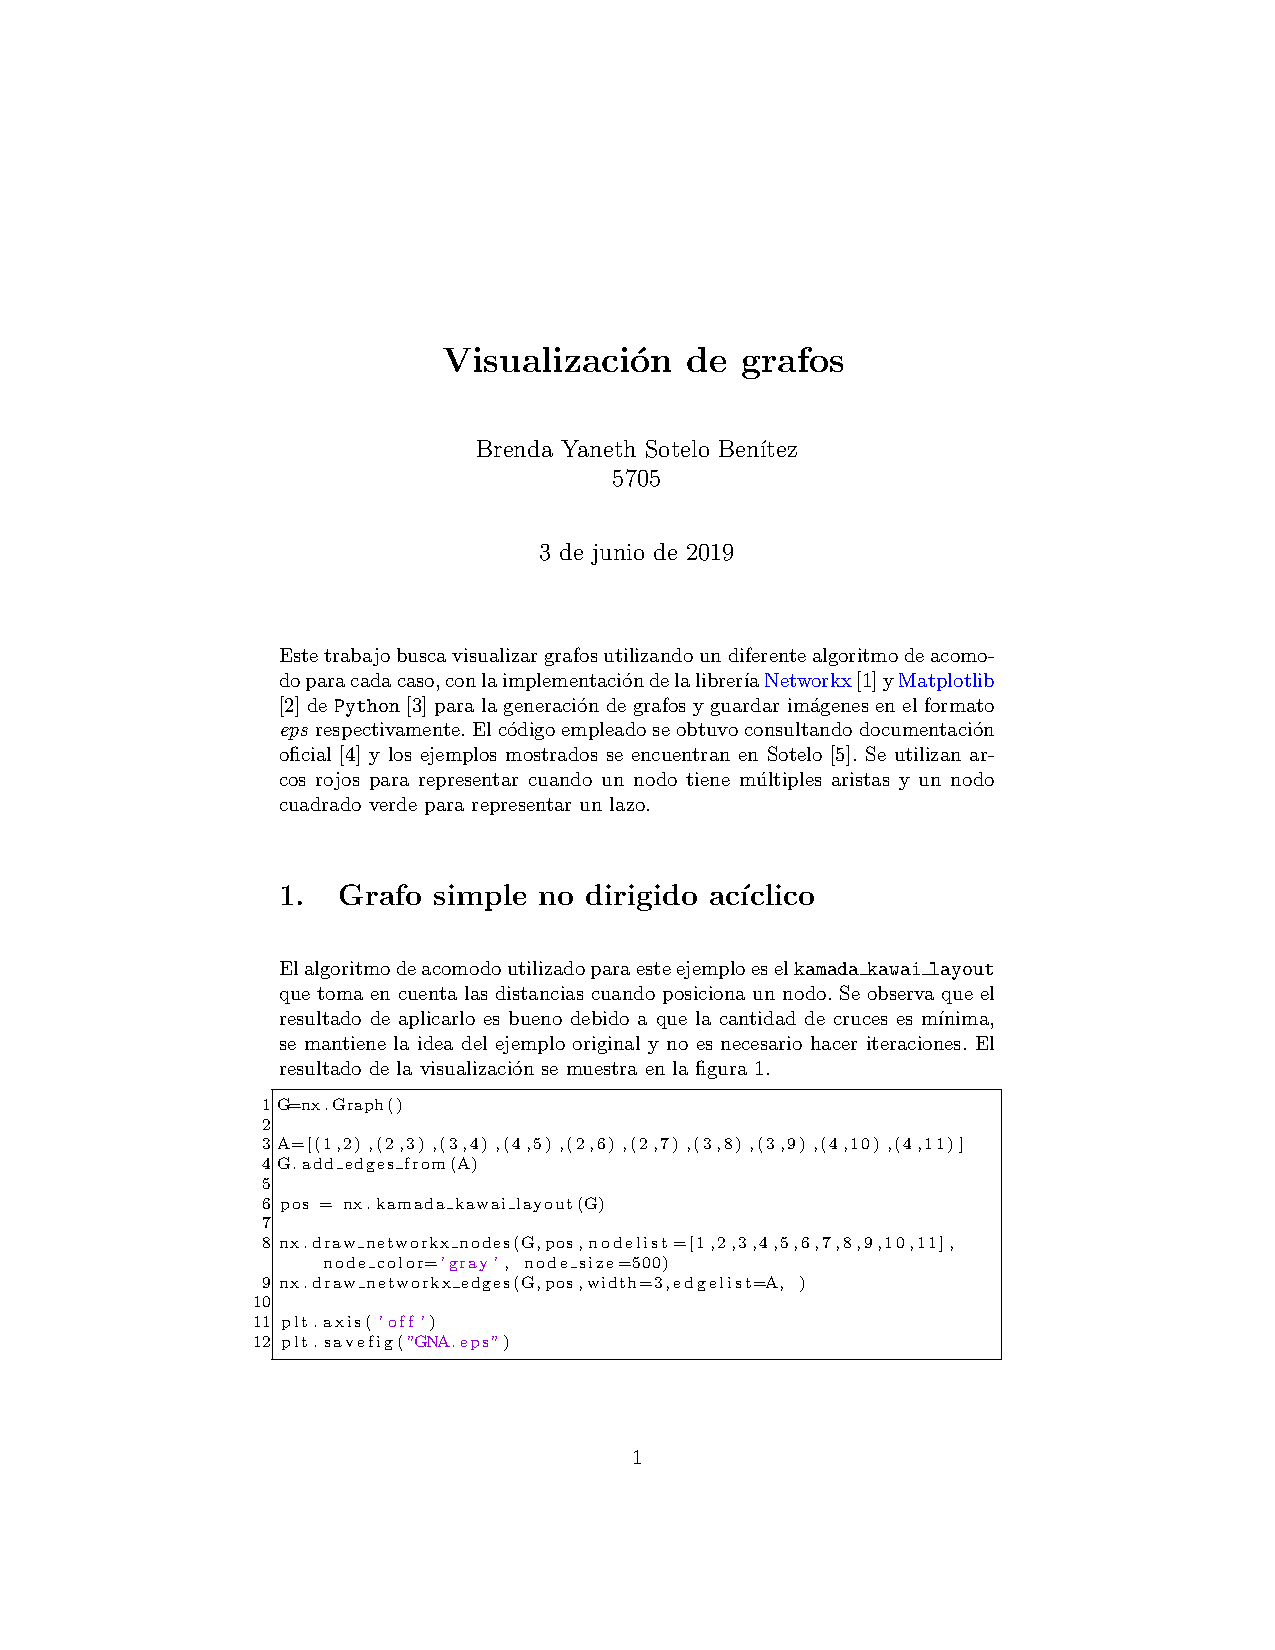
\includepdf[pages=-]{Tarea2_FR.pdf}
%---------------------------------------------------------

%---------------------------------------------------------
\section*{Tarea 3}

En esta práctica se realizaron pequeñas correcciones ortográficas y en las tablas, donde se ajusto la orientación de los valores a la derecha y que tuvieran todos la misma cantidad de decimales. Aún así se muestra la versión corregida de la tarea. 

\newpage
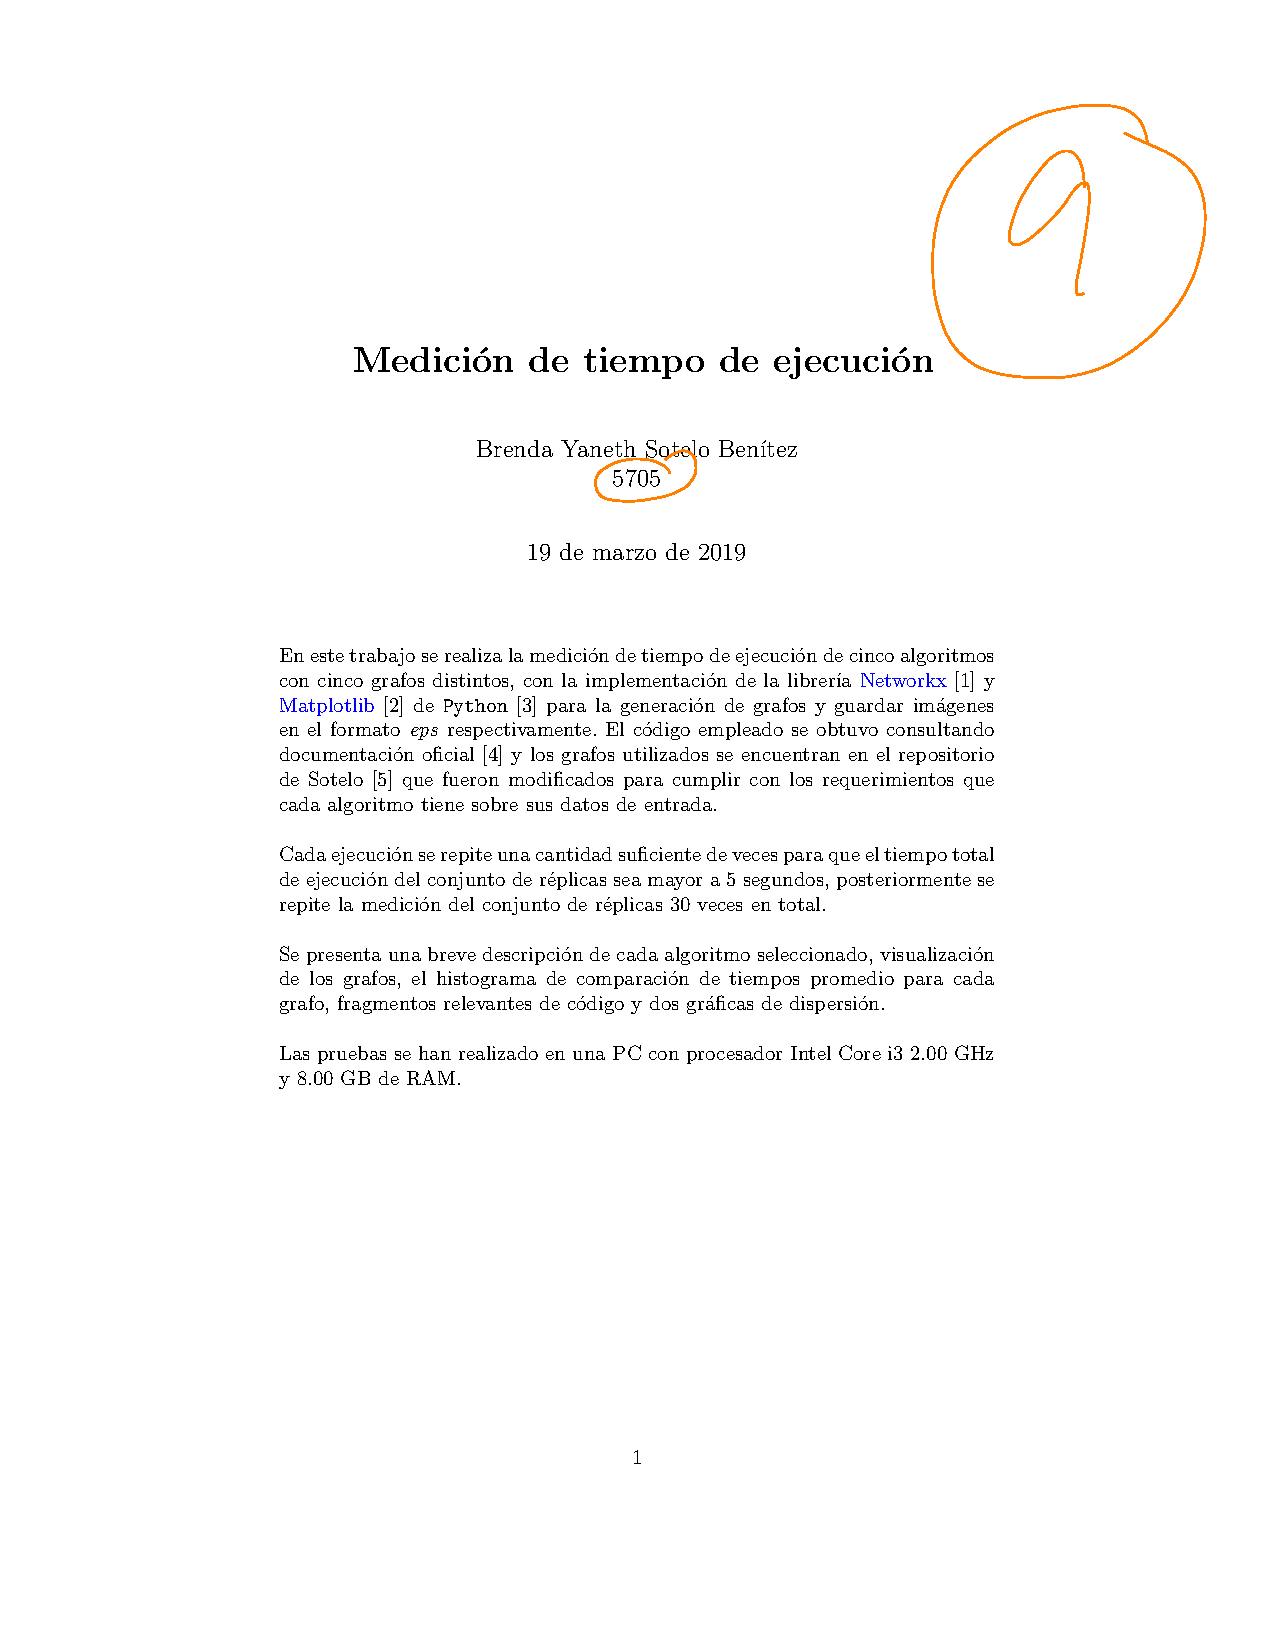
\includepdf[pages=-]{5705-3.pdf}
\newpage
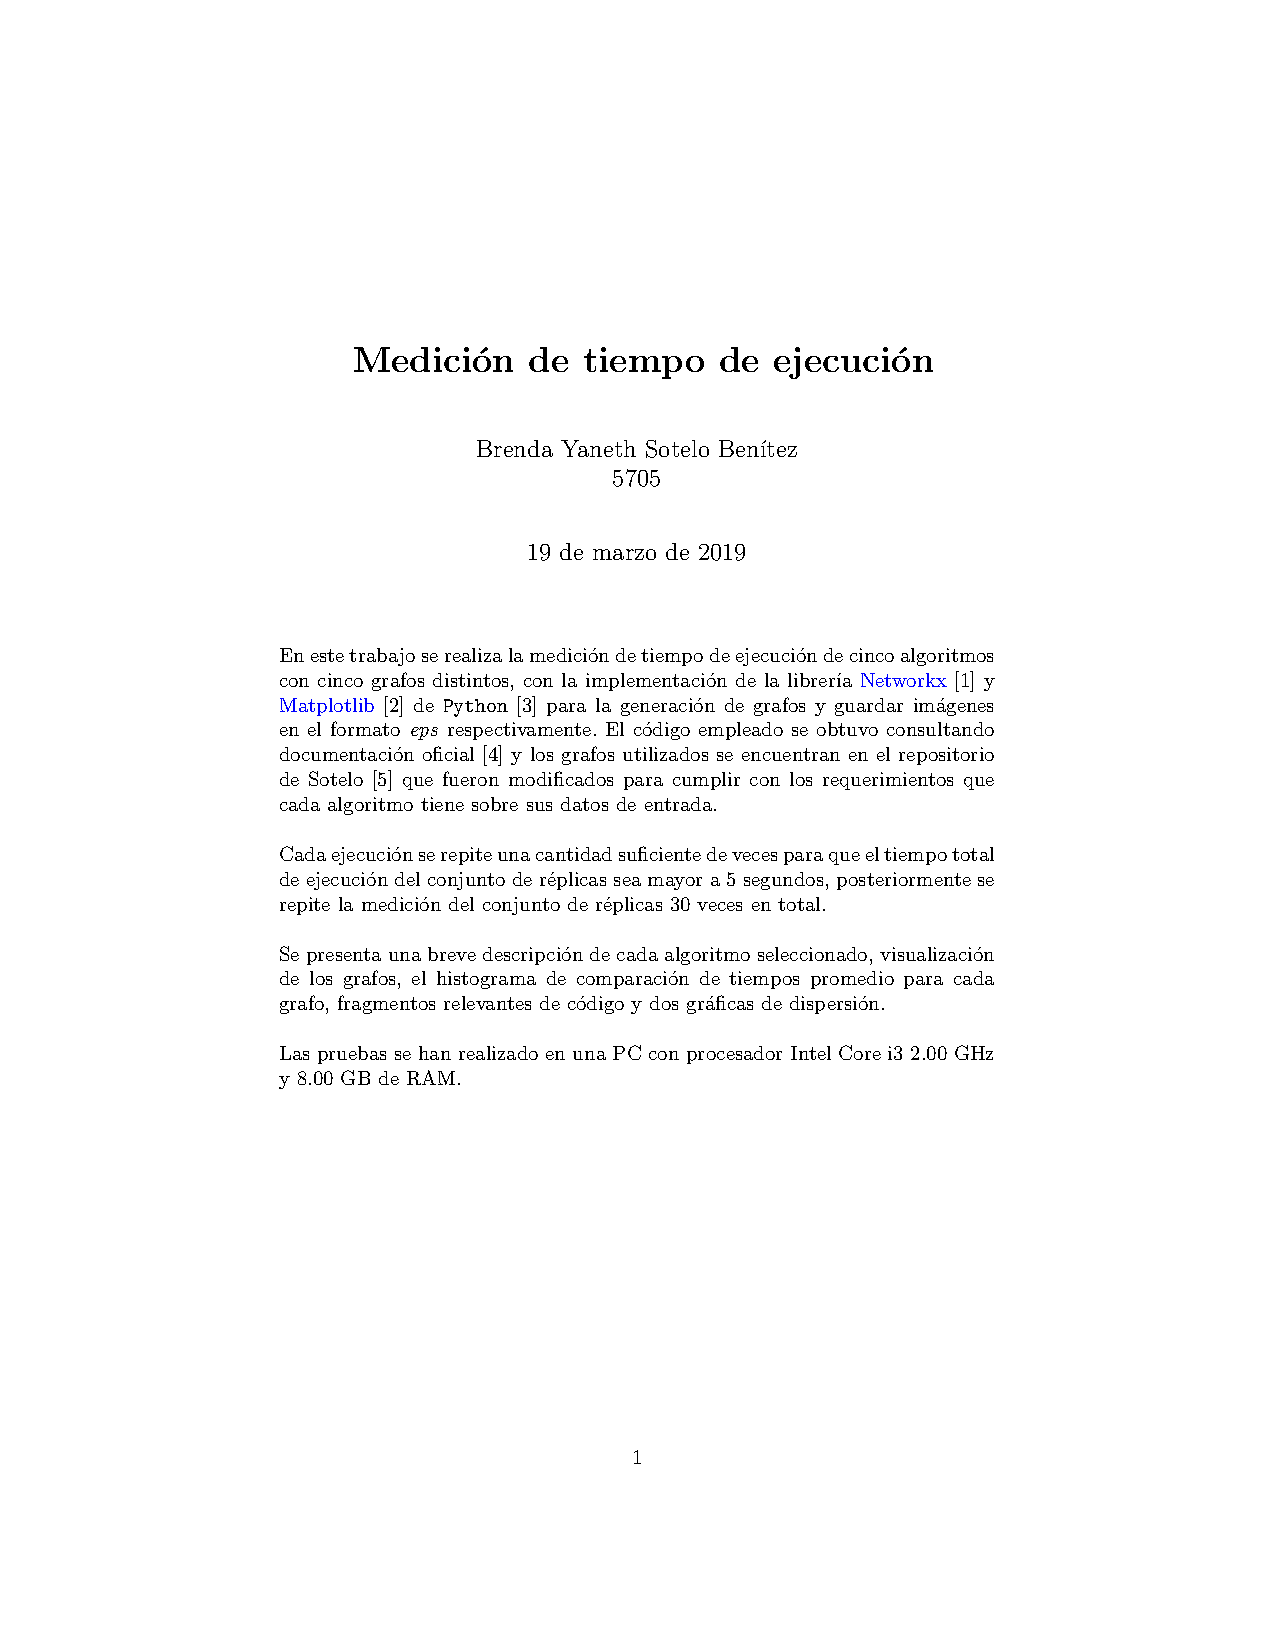
\includepdf[pages=-]{Tarea3_FR.pdf}
%---------------------------------------------------------

%---------------------------------------------------------
\section*{Tarea 4}

En esta práctica se realizaron correcciones ortográficas y de ausencia de código. 

\newpage
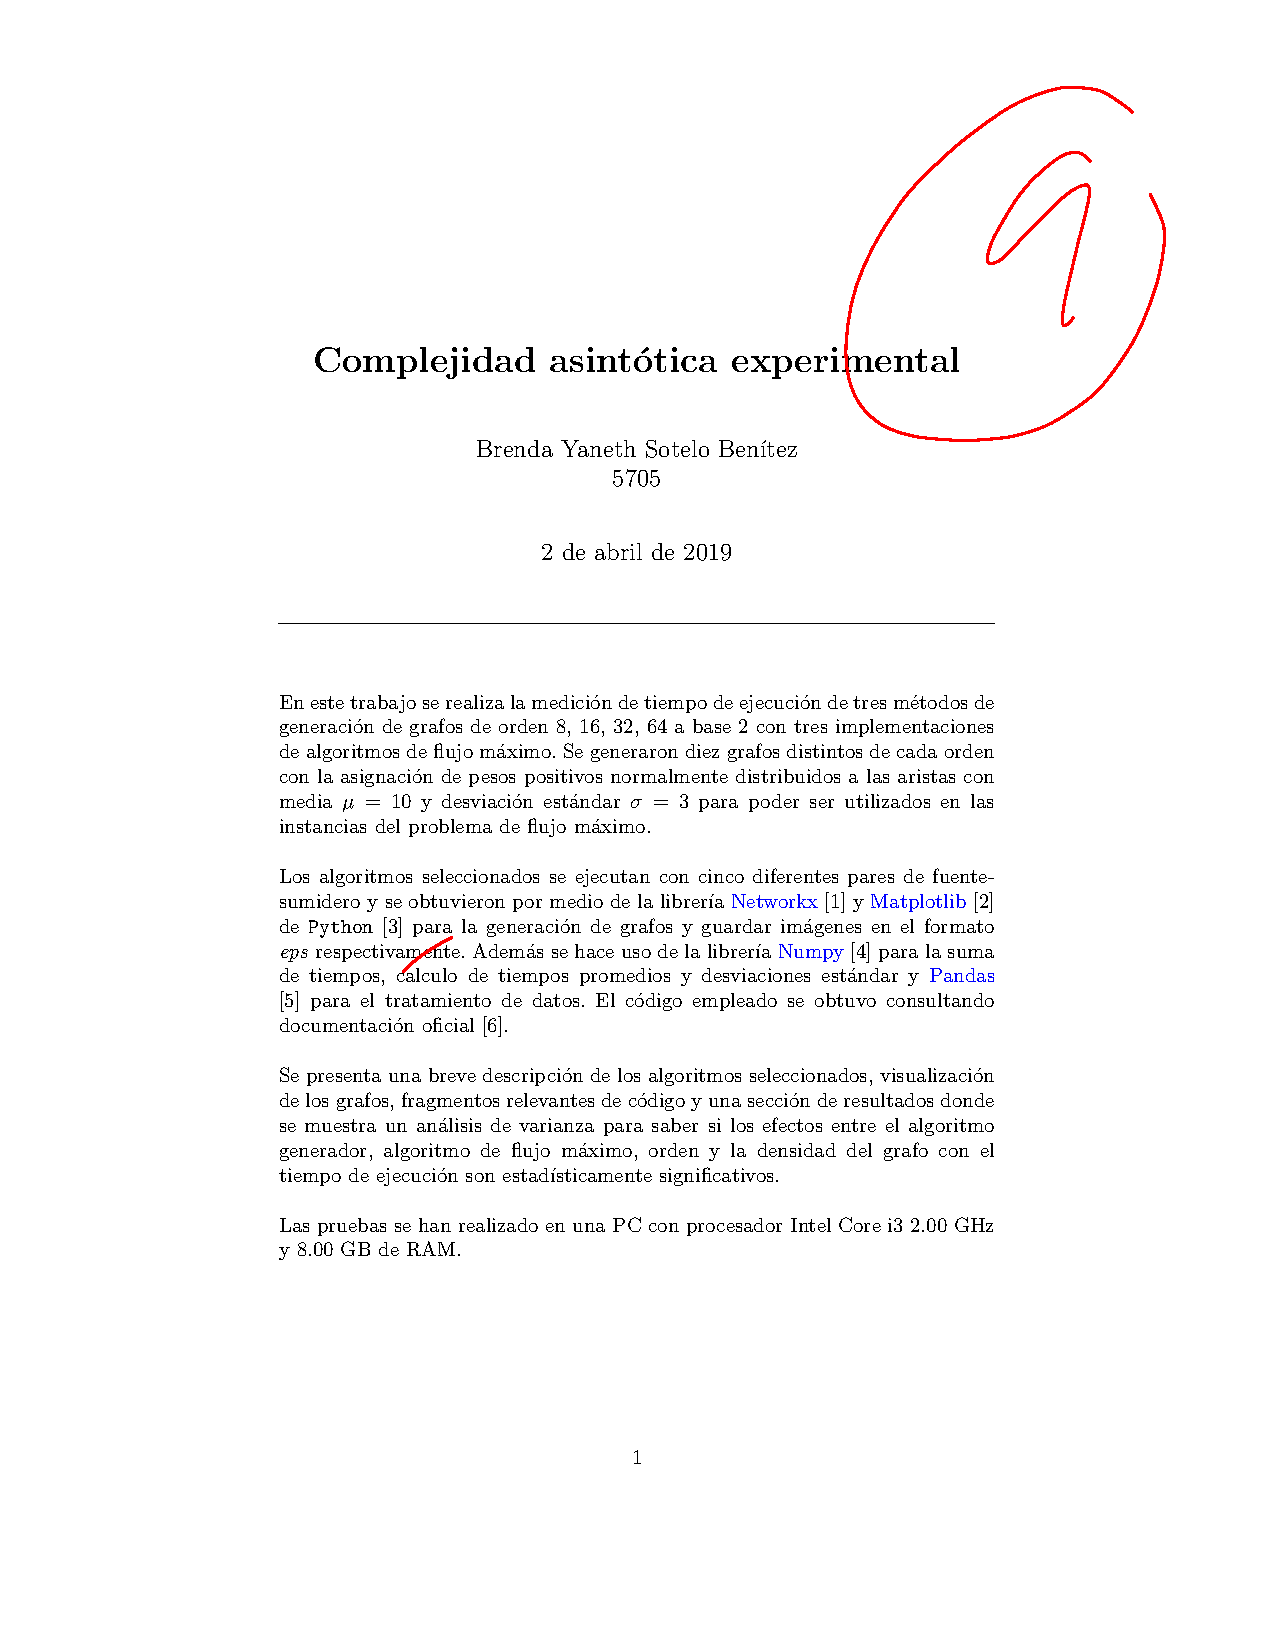
\includepdf[pages=-]{5705-4.pdf}
\newpage
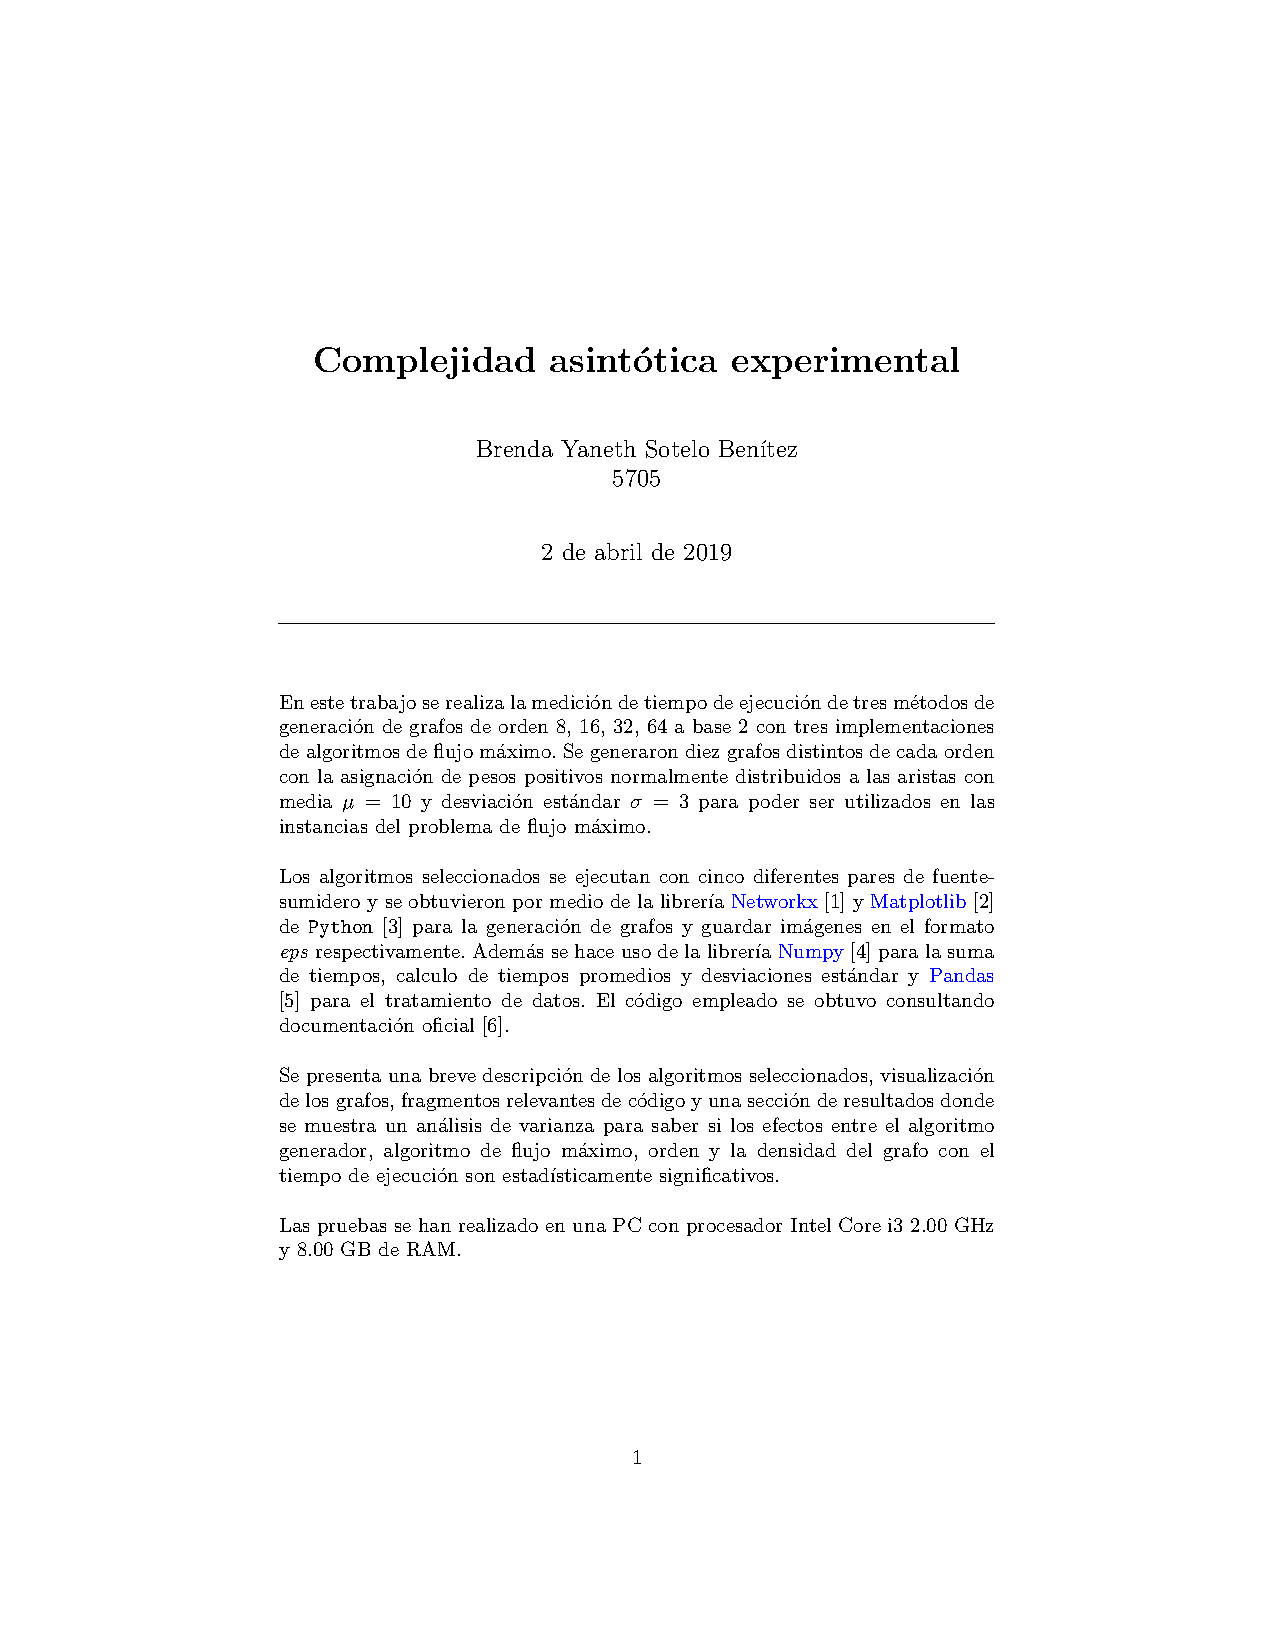
\includepdf[pages=-]{Tarea4_FR.pdf}
%---------------------------------------------------------

%---------------------------------------------------------
\section*{Tarea 5}

Para esta práctica se realizaron correcciones ortográficas y detalles en las gráficas que se utilizaron. 

\newpage
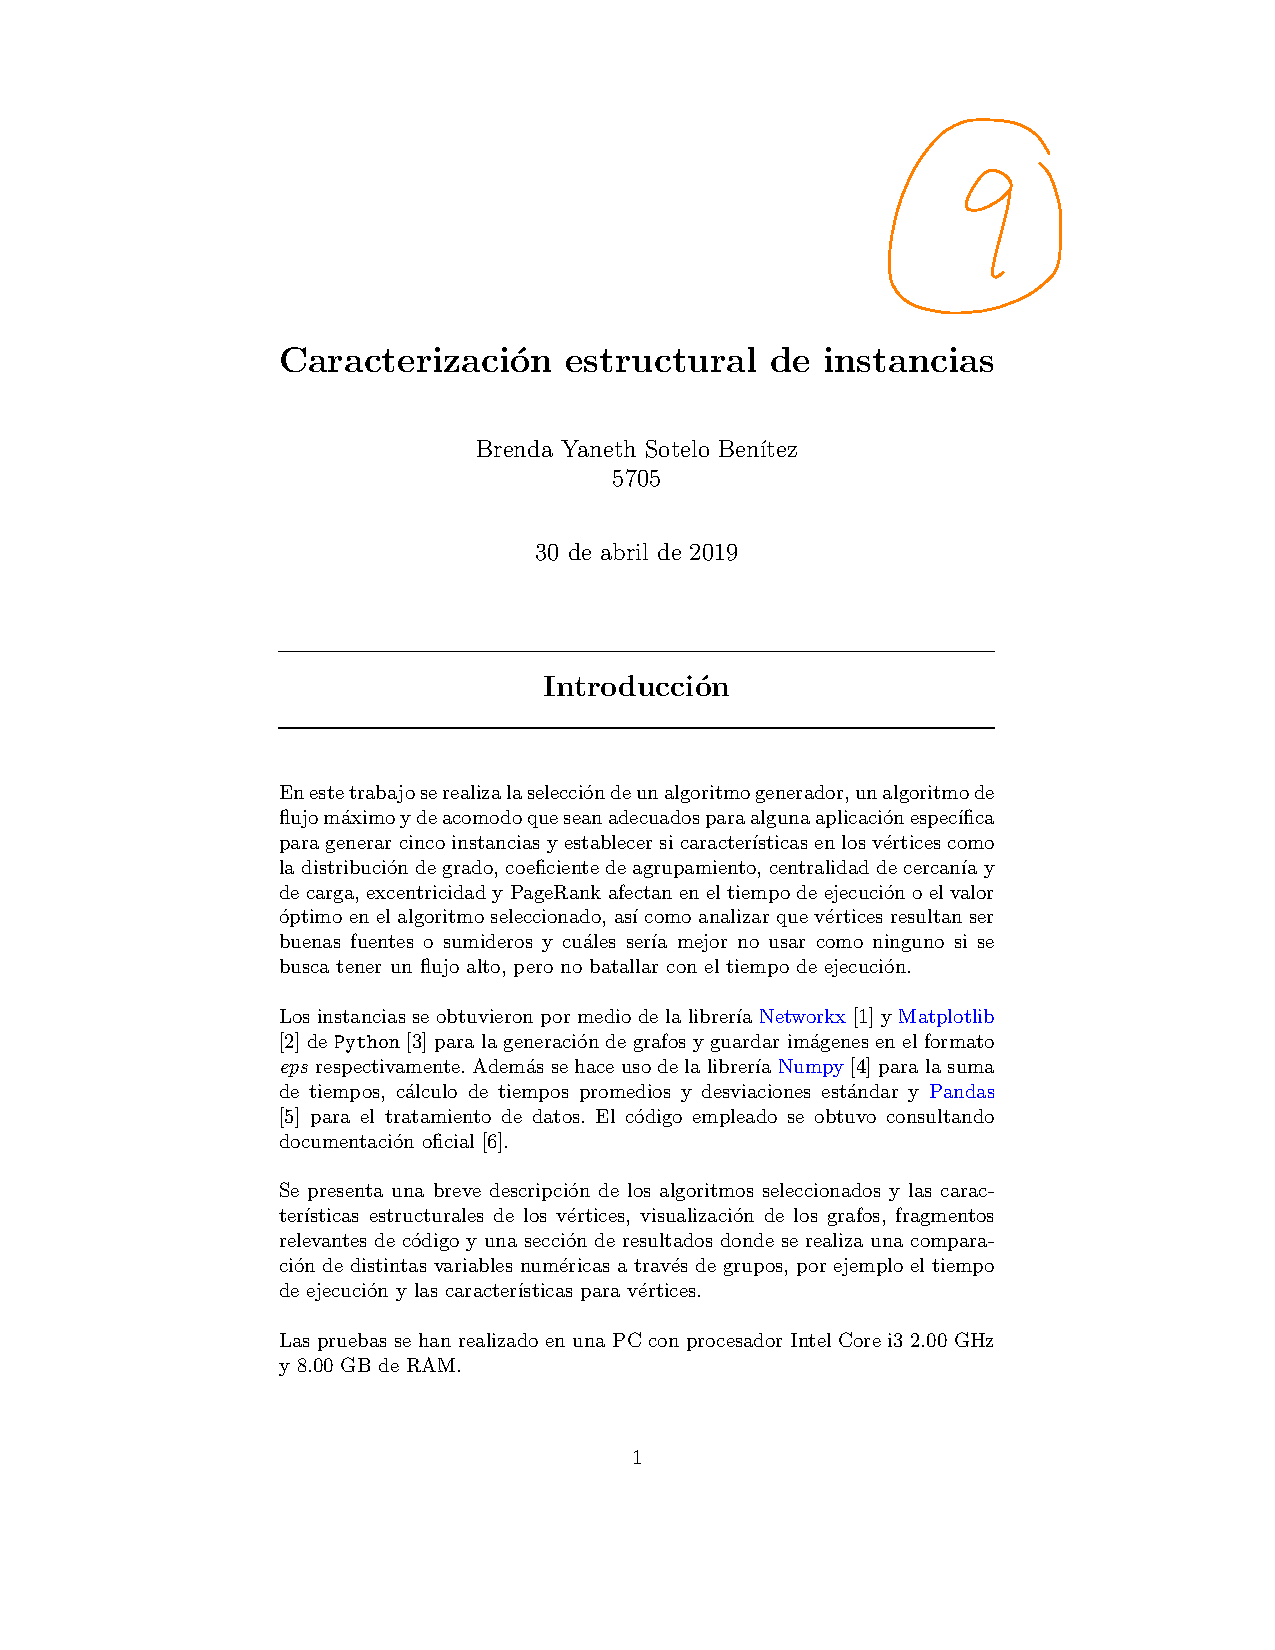
\includepdf[pages=-]{5705-5.pdf}
\newpage
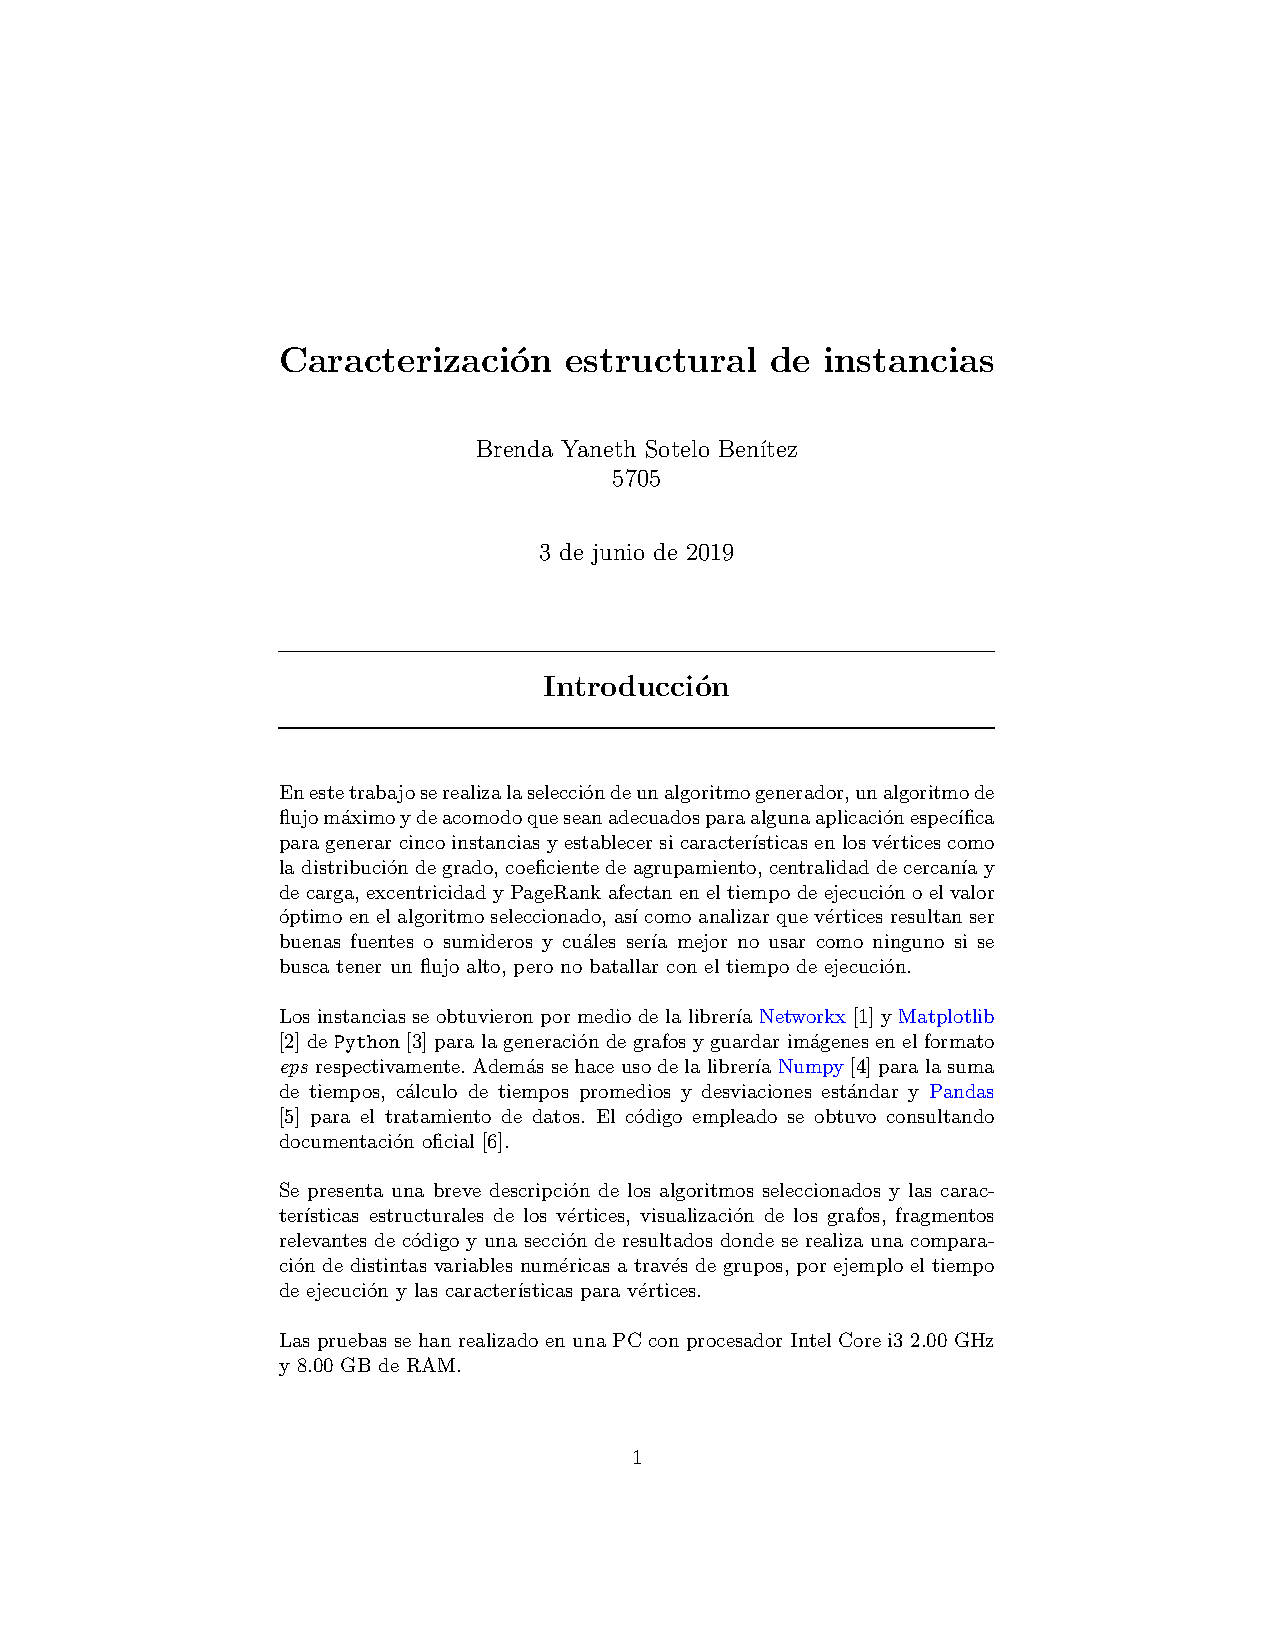
\includepdf[pages=-]{Tarea5_FR.pdf}
%---------------------------------------------------------

%---------------------------------------------------------
\section*{Tarea 6}

Finalmente se incluye la tarea 6 que no consta de un archivo con correcciones. 

\newpage
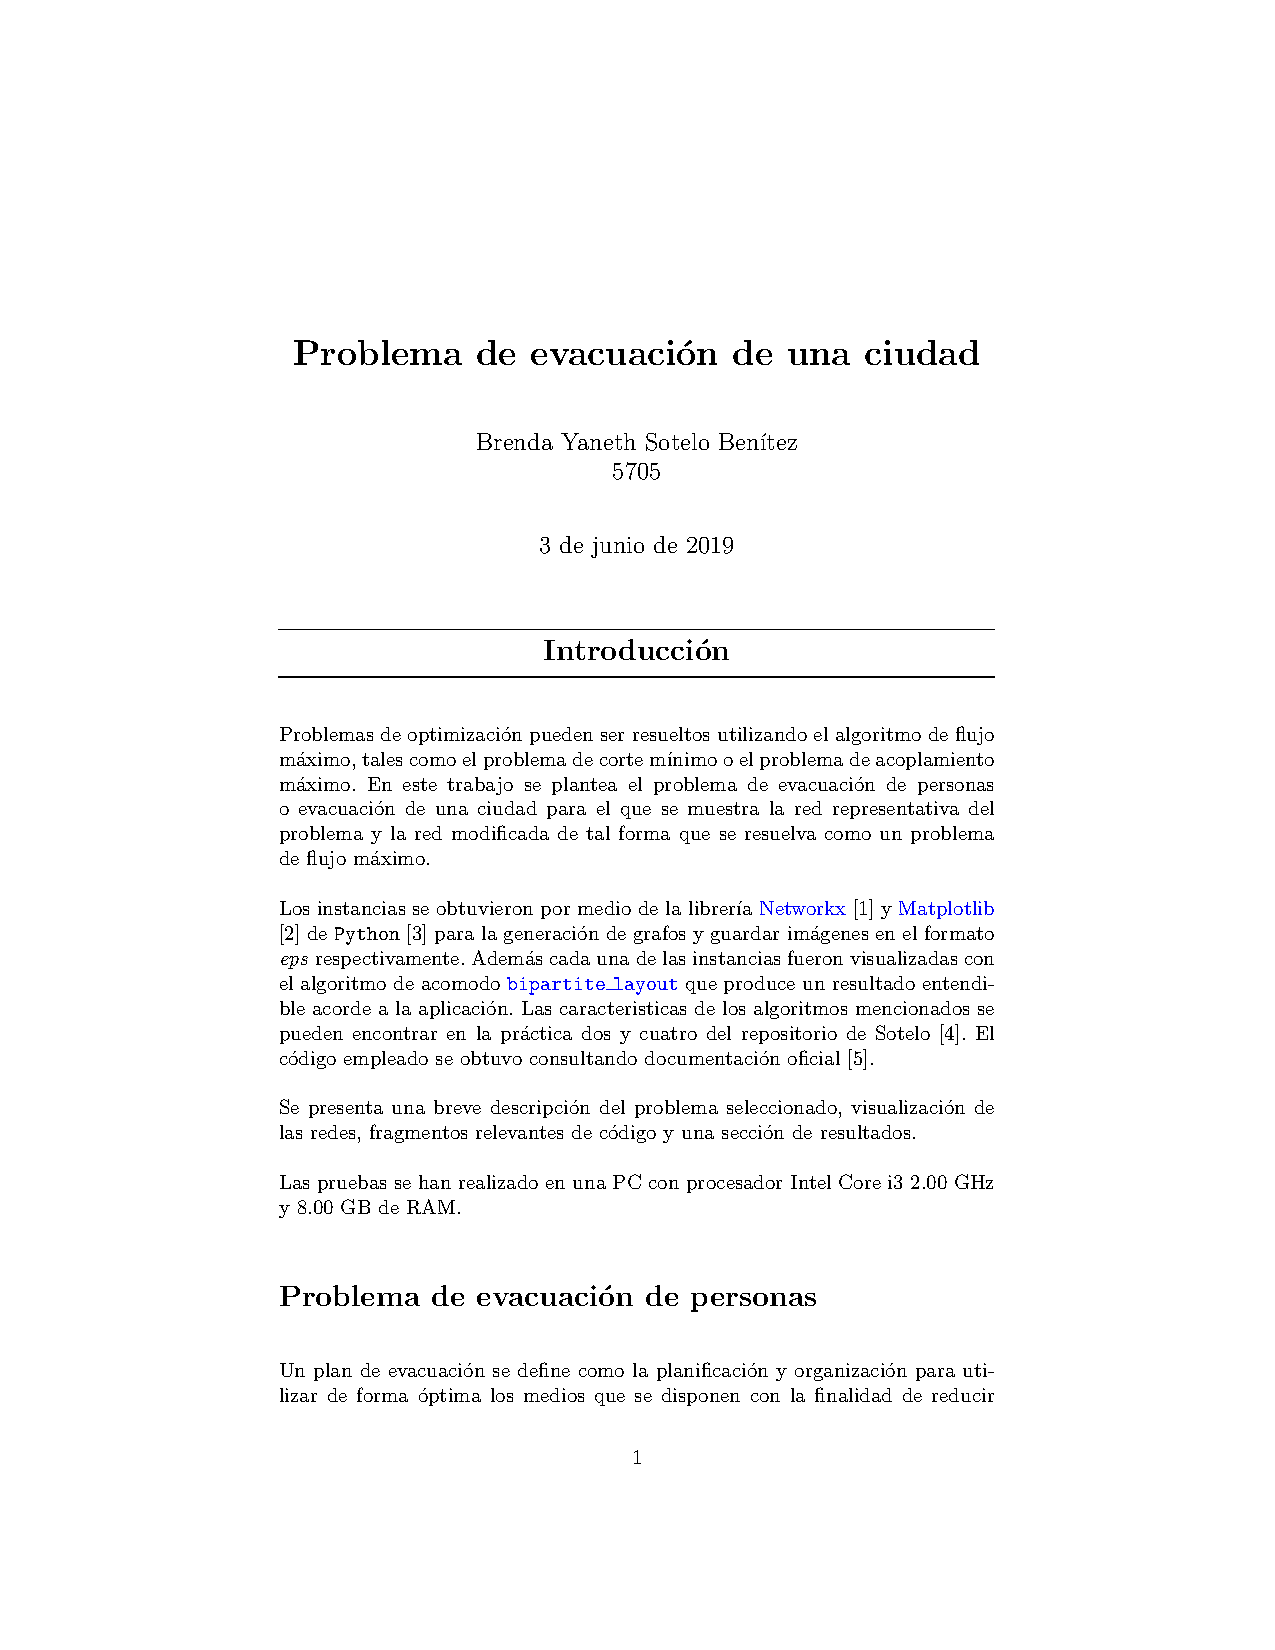
\includepdf[pages=-]{5705-6.pdf}
%---------------------------------------------------------
\end{document}